\documentclass[5p]{elsarticle}       			% 5p gir 2 kolonner pr side. 1p gir 1 kolonne pr side.
\journal{professor}
\usepackage{graphicx}       			      	% For Πinkludere figurer.
\usepackage{amsmath,amssymb} 			% Ekstra matematikkfunksjoner.
\usepackage[font=small,labelfont=bf]{caption}	% For justering av figurtekst og tabelltekst.
\usepackage[export]{adjustbox}           		% for Œ kunne plassere figurer bedre, h¿yre venstre justering
\usepackage{hyperref}					% For å skrive webadresser

% Disse kommandoene kan gj¿re det enklere for LaTeX Œ plassere figurer og tabeller der du ¿nsker.
\setcounter{totalnumber}{5}
\renewcommand{\textfraction}{0.05}
\renewcommand{\topfraction}{0.95}
\renewcommand{\bottomfraction}{0.95}
\renewcommand{\floatpagefraction}{0.35}

%%%%%%%%%%%%%%%%%%%%%%%%%%%%%%%%%%%%%%%%%%%%%%%%%%%%%%%%%%%%%%%%%%%%%%%%%
\begin{document}

\begin{frontmatter}


\title{Numerical Solution of the Schr\"{o}dinger Equation}
\author[fysikk]{H\aa kon Task\'{e}n}
\author[fysikk]{Paul Thrane}
\address[fysikk]{Institute for Physics, Norwegian University of Science and Technology, N-7491 Trondheim, Norway.}

\begin{abstract}
We have written a program that integrates the Schr\"{o}dinger equation numerically, thereby finding how a system evolves given a time independent potential and an initial state. The solution works both for one and two dimensional systems.
\end{abstract}

\end{frontmatter}


%%%%%%%%%%%%%%%%%%%%%%%%%%%%%%%%%%%%%%%%%%%%%%%%%%%%%%%%%%%%%%%%%%%%%%%%%
\section{The program}
The program is composed of two major parts, schrodin-gerFD and plotSchrodinger.py. schrodingerFD is implemented using C++, and is used to make the initial state, determine the time evolution of the system by integrating the Schr\"{o}dinger equation using finite differences, as well as saving these results in certain files. plotSchrodinger.py is implemented in python, and is used to make an animated movie of the progress of the system\cite{jake}. In addition to these programs, there are several .txt files that are needed to run a simulation; also, several shell scripts have been made to automate the process. For information on how to run a simulation, see README.md\footnote{Note that to run plotSchrodinger.py as included, ffmpeg must be installed. An alternative is to modify plotSchrodinger.py as described in the code.}. All of these files should be included with this document, but can also be found at \url{https://github.com/task123/schrodingerFD}.

%%%%%%%%%%%%%%%%%%%%%%%%%%%%%%%%%%%%%%%%%%%%%%%%%%%%%%%%%%%%%%%%%%%%%%%%%
\section{Results}
The program works well for the different conditions tested, and can easily be expanded to include new potentials and initial conditions. To view the results of a few simulations, a couple of output .mp4 files have been placed in the subdirectory simulationMovies. For the specific situations described in problem 4 and 5 in \cite{exercise}, the probability of reflection and transmission was calculated for varying potential height and width, respectively. The results are shown in figure \ref{oppg4} and \ref{oppg5}.
\begin{figure}[h] 
	\begin{center}
		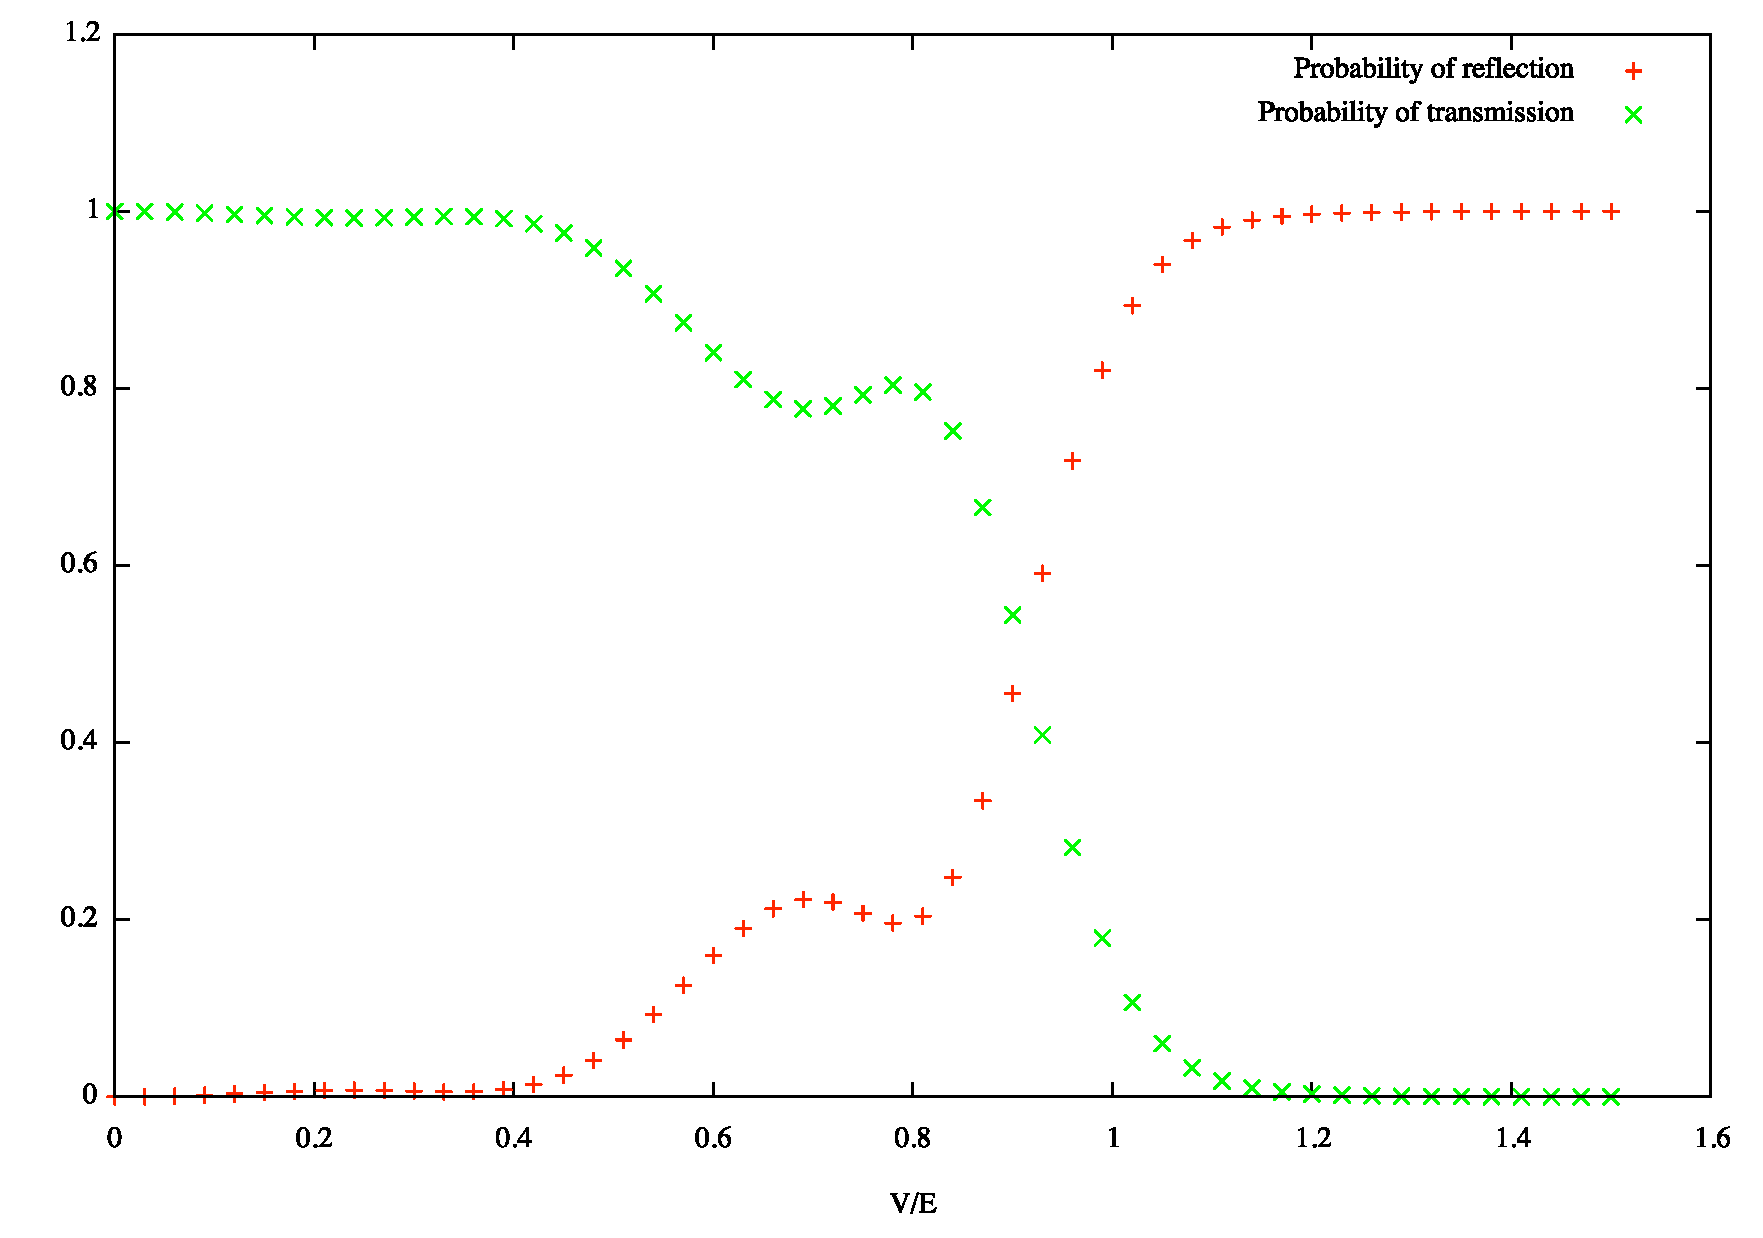
\includegraphics[width=.5\textwidth,center]{oppgave4.pdf} 
	\end{center}
		\caption{Probability of transmission and reflection for a wave packet traveling towards a square potential in one dimension, as described in problem 4 in \cite{exercise}.} 
		\label{oppg4}
\end{figure}
\begin{figure}[h] 
	\begin{center}
		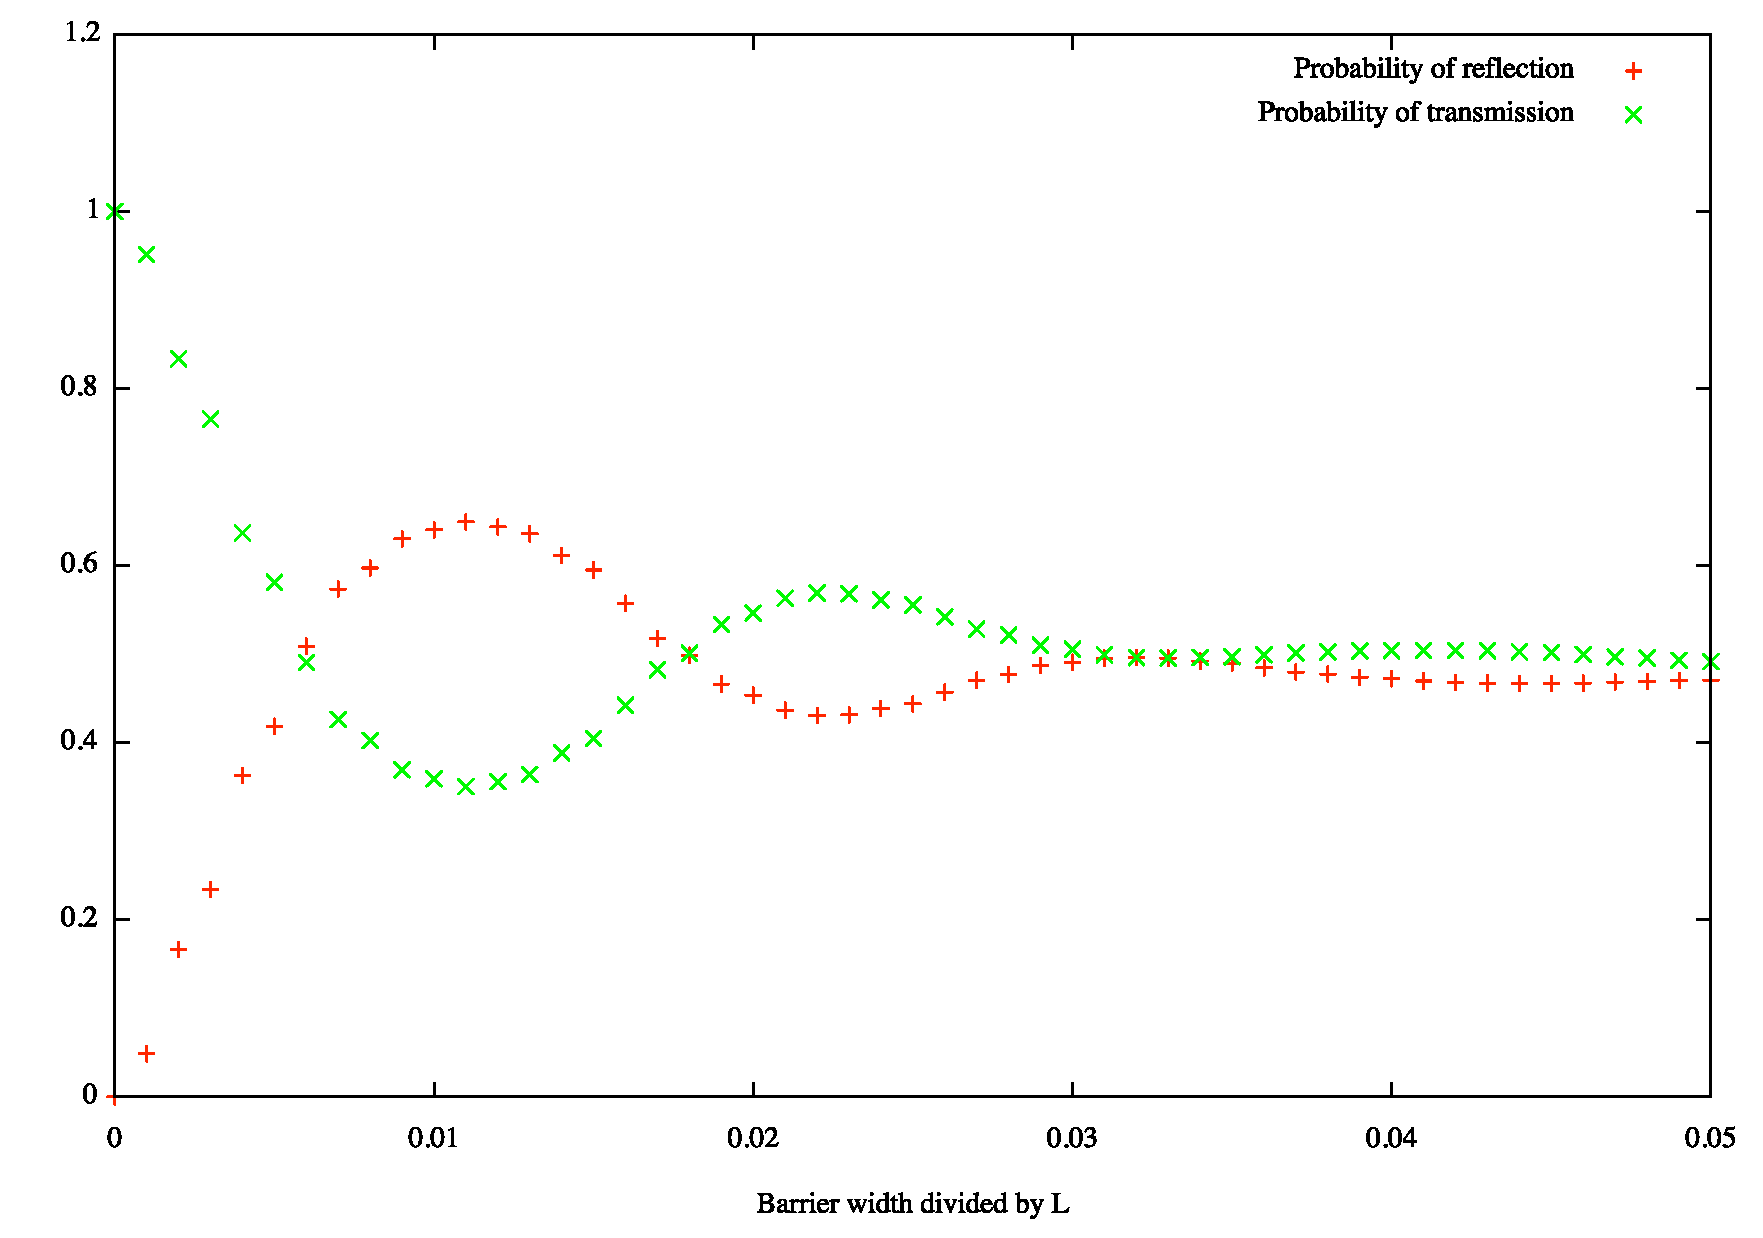
\includegraphics[width=.5\textwidth,center]{oppgave5.pdf} 
	\end{center}
		\caption{Probability of transmission and reflection for a wave packet traveling towards a square potential in one dimension, as described in problem 5 in \cite{exercise}. Here, $L$ is the lengt of the system.} 
		\label{oppg5}
\end{figure}

%%%%%%%%%%%%%%%%%%%%%%%%%%%%%%%%%%%%%%%%%%%%%%%%%%%%%%%%%%%%%%%%%%%%%%%%%
\section*{References}

\begin{thebibliography}{99}

\bibitem{exercise}
Institute for Physics, NTNU. Numerical exercise FY2045 Quantum Mechanics, Fall 2015. Available from \url{http://amokk.phys.ntnu.no/files/FY2045_2015/exercise15/numerics.pdf}

\bibitem{jake}
Jake Vanderplas. Matplotlib Animation Tutorial, August 18, 2012. Available from \url{https://jakevdp.github.io/blog/2012/08/18/matplotlib-animation-tutorial/}


\end{thebibliography}

\end{document}
